\exercisesection{COHEN RINGS}

In the exercises of § 2, \(p\) is a fixed prime number. If \(a\) is an ideal of a ring A, we denote by \(a^p\) the ideal generated by the elements \(a^p\) , where \(a\) ranges over \(a\) .

\begin{enumerate}
\def\labelenumi{\arabic{enumi})}
\item
  Let \((\mathbf{C}_{n}, \pi_{n,m})\) be a projective system of rings relative to the index set N. We assume that \(C_{n}\) is Artinian for every \(n \in N\) and that the homomorphisms \(\pi_{n,m}\) are surjective. Let \(\pi_{n}\) be the canonical homomorphism from \(C = \varprojlim C_{n}\) into \(C_{n}\). Show that for all \(x \in C\), one has \(xC = \varprojlim \pi_{n}(x) C_{n}\). (Proceed as in the proof of Prop. 3 of § 2, no. 1.)
\item
  Let A be a ring and \((\mathbf{J}_{n})_{n\in\mathbb{N}}\) a decreasing sequence of ideals of A, such that \(pJ_{n} + J_{n}^{p} \subset J_{n+1}\) for every \(n \in N\).
\end{enumerate}

\begin{enumerate}
\def\labelenumi{\alph{enumi})}
\item
  Prove that the assertions of Lemma 1 and Prop. 1 of § 1, no. 1 are still true under this hypothesis.
\item
  Let \(i\) and \(n\) be two positive integers. When \(i \leqslant n\), the map \(x \mapsto p^i x^{p^n - i}\) from A to A defines, by passing to quotients, a map
\end{enumerate}

\[
\rho_ {n, i} ^ {\mathbf {A}}: \mathrm{A} / \mathrm{J} _ {0} \rightarrow \mathrm{A} / \mathrm{J} _ {n}.
\]

For \(i > n\) , we set \(\rho_{n,i}^{\mathbf{A}} = 0\) . For \(x \in \mathrm{A} / \mathrm{J}_n\) and \(a \in \mathrm{A} / \mathrm{J}_0\) , one has \(x^{p^{n - i}} \rho_{n,i}^{\mathbf{A}}(a) = \rho_{n,i}^{\mathbf{A}}(\overline{x} a)\) , where \(\overline{x}\) is the image of \(x\) in \(\mathrm{A} / \mathrm{J}_0\) . If \(j\) is a positive integer and that \(a, b\) are two elements of \(\mathrm{A} / \mathrm{J}_n\) , one has

\[
\rho_ {n, i} ^ {\mathbf {A}} (a) \rho_ {n, j} ^ {\mathbf {A}} (b) = \rho_ {n, i + j} ^ {\mathbf {A}} \left(a ^ {p ^ {j}} b ^ {p ^ {i}}\right).
\]

\begin{enumerate}
\def\labelenumi{\alph{enumi})}
\setcounter{enumi}{2}
\tightlist
\item
  Let \((\mathbf{R}_{n})_{n\in\mathbf{N}}\) be the sequence of polynomials constructed in exerc. 3, p.~42. Let n and i be two positive integers, and let a and b be two elements of \(A/J_{0}\). We then have, in \(A/J_{n}\), the equality
\end{enumerate}

\[
\rho_ {n, i} ^ {\mathrm{A}} (a) + \rho_ {n, i} ^ {\mathrm{A}} (b) = \sum_ {m = 0} ^ {n - i} \rho_ {n, i + m} ^ {\mathrm{A}} (\mathrm{R} _ {m} (a, b)).
\]

\begin{enumerate}
\def\labelenumi{\arabic{enumi})}
\setcounter{enumi}{2}
\tightlist
\item
  Let \(n\) be a positive integer. Let C be a \(p\)-Cohen ring, with residue field \(k\), and of length \(n+1\). Let \((x_{\lambda})_{\lambda\in\Lambda}\) be a family of elements of C lifting a \(p\)-basis \((\xi_{\lambda})_{\lambda\in\Lambda}\) of \(k\). We denote by \(\rho_{i}:k\to C\), for every \(i\in\mathbf{N}\), the map \(\rho_{n,i}^{\mathrm{C}}\) defined in Exerc. 2, where one takes for \(\mathbf{J}_{m}\) the ideal \(p^{m+1}\mathbf{C}\).
\end{enumerate}

\begin{enumerate}
\def\labelenumi{\alph{enumi})}
\tightlist
\item
  For \(r \in \mathbf{N}\), let \(\mathbf{M}_r\) be the set of multi-indices \(m \in \mathbf{N}^{(\Lambda)}\) such that, for every \(\lambda \in \Lambda\), one has \(0 \leqslant m_{\lambda} < p^{r}\). Then, for every element \(\alpha\) of C, there exists a unique finitely supported family \((a_{i,m})\) (\(0 \leqslant i \leqslant n\), \(m \in \mathbf{M}_{n-i}\)) of elements of \(k\), such that
\end{enumerate}

\[
\alpha = \sum_ {i = 0} ^ {n} \sum_ {m \in \mathbf {M} _ {n - i}} \rho_ {i} (a _ {i, m}) x ^ {m},
\]

where the notation \(x^{m}\) denotes the product \(\prod x_{\lambda}^{m_{\lambda}}\) .

\begin{enumerate}
\def\labelenumi{\alph{enumi})}
\setcounter{enumi}{1}
\tightlist
\item
  Consider the ring U generated by the generators \([x_{\lambda}]\), with \(\lambda\) ranging over \(\Lambda\), and \([\rho_{i}(a)]\), with i ranging over N and a ranging over k, and subject only to the following relations (where the polynomials \(R_{i}\) are those introduced in Exerc. 3, p.~42).
\end{enumerate}

\begin{enumerate}
\def\labelenumi{(\roman{enumi})}
\item
  \([\rho_i(a)] = 0\) for \(a \in k, i > n\) ,
\item
  \(\left[\rho_0(1)\right] = 1\) and \(\left[\rho_0(0)\right] = 0,\)
\item
  \([\rho_i(a)][\rho_j(b)] = [\rho_{i + j}(a^{p^j}b^{p^i})]\) for \(i,j\) in \(\mathbf{N}\) and \(a,b\) in \(k\) ,
\item
  \([\rho_i(a)] + [\rho_i(b)] = \sum [\rho_{i+m}(\mathbf{R}_m(a,b))]\) for \(i\in \mathbf{N}\) and \(a,b\) in \(k,\)
\item
  \([x_{\lambda}]^{p^{n - i}}[\rho_i(a)] = [\rho_i(\xi_{\lambda}a)]\) for \(0 \leqslant i \leqslant n, \lambda \in \Lambda, a \in k\) .
\end{enumerate}

Prove that we have \([\rho_i(0)] = 0\) for every \(i \in \mathbf{N}\) .

Prove, using exercise 3, b), p.~42, that if \(p\) is odd, we have \([\rho_0(-1)] = -1\) ; if \(p\) is even, we have \(\sum_{i=0}^{n} [\rho_i(1)] = -1\) .

\begin{enumerate}
\def\labelenumi{\alph{enumi})}
\setcounter{enumi}{2}
\tightlist
\item
  There exists a unique map from U to C which, for every finitely supported family \((a_{i,m})_{0\leqslant i\leqslant n,m\in M_{n - i}}\) of elements of \(k\) associated with the element
\end{enumerate}

\[
\left\langle \left(a _ {i, m}\right) \right\rangle = \sum_ {i = 0} ^ {n} \sum_ {m \in \mathbf {M} _ {n - i}} \left[ \rho_ {i} (a _ {i, m}) \right] \prod_ {\lambda \in \Lambda} [ x _ {\lambda} ] ^ {m _ {\lambda}}
\]

of U the element \(\sum_{i=0}^{n}\sum_{m\in M_{n-i}}\rho_i(a_{i,m})x^m\) of C; it is a ring isomorphism.

\begin{enumerate}
\def\labelenumi{\alph{enumi})}
\setcounter{enumi}{3}
\tightlist
\item
  Deduce from the foregoing another proof of the results of § 2, no. 3.
\end{enumerate}

\begin{enumerate}
\def\labelenumi{\arabic{enumi})}
\setcounter{enumi}{3}
\tightlist
\item
  Let C be a \(p\)-Cohen ring of infinite length, and \(k\) its residue field. Let A be a ring, and \((\mathbf{J}_n)_{n \in \mathbb{N}}\) a decreasing sequence of ideals of A satisfying \(p\mathbf{J}_n + \mathbf{J}_n^p \subset \mathbf{J}_{n+1}\) for every \(n \in \mathbb{N}\). Finally, let \(\overline{\varphi}: k \to \mathrm{A} / \mathrm{J}_0\) be a ring homomorphism, \((\xi_\lambda)_{\lambda \in \Lambda}\) a \(p\)-basis of \(k\), \((x_\lambda)_{\lambda \in \Lambda}\) a family of elements of C lifting this \(p\)-basis, and \((a_\lambda)_{\lambda \in \Lambda}\) a family of elements of A, such that the image of \(a_\lambda\) in \(\mathrm{A} / \mathrm{J}_0\) is \(\overline{\varphi}(\xi_\lambda)\).
\end{enumerate}

\begin{enumerate}
\def\labelenumi{\alph{enumi})}
\item
  For every \(n\in\mathbf{N}\), there exists a unique homomorphism \(\varphi_{n}\) from \(\mathrm{C}/p^{n+1}\mathrm{C}\) into \(\mathrm{A}/\mathrm{J}_{n}\) such that \(\varphi_{n}\circ\rho_{n,i}^{\mathrm{C}}=\rho_{n,i}^{\mathrm{A}}\circ\overline{\varphi}\) and such that the image under \(\varphi_{n}\) of the class of \(x_{\lambda}\) is the class of \(a_{\lambda}\) (Use Exercises 2 and 3.)
\item
  Suppose that A is separated and complete for the topology defined by the filtration \((\mathrm{J}_{n})_{n\in\mathbb{N}}\). Then there exists a unique ring homomorphism \(\varphi\) from C to A, such that \(\varphi(x_{\lambda}) = a_{\lambda}\) for \(\lambda \in \Lambda\), and that \(\varphi\) induces \(\overline{\varphi}\) by passing to quotients. This homomorphism is continuous.
\item
  Suppose that the ring A is local, separated, and complete, that one has \(J_{n} = m_{A}^{n+1}\) for every \(n \in N\), that one has \(A/J_{0} = k\), and that \(\overline{\varphi}\) is the identity map. Prove that the image under \(\varphi\) of C in A is the unique Cohen subring of \(A'\) containing each of the elements \(a_{\lambda}\), and thus give another proof of part a) of th. 1 of § 2, no. 2; if k is perfect and C is the ring W(k), one obtains another proof of th. 2 of § 2, no. 4.
\end{enumerate}

\begin{enumerate}
\def\labelenumi{\arabic{enumi})}
\setcounter{enumi}{4}
\tightlist
\item
  Let A be a ring and \((\mathrm{J}_n)_{n\in \mathbb{N}}\) a decreasing sequence of ideals of A, satisfying \(p\mathbf{J}_n + \mathbf{J}_n^p\subset \mathbf{J}_{n + 1}\) for every integer \(n\geqslant 0\). Let R be a ring of characteristic \(p\) and \(\overline{\varphi}\) a ring homomorphism from R to \(\mathrm{A} / \mathrm{J}_0\). One calls a lifting of \(\overline{\varphi}\) into \(\mathrm{A} / \mathrm{J}_n\) a map \(\varphi_n:\mathbb{R}\to \mathbb{A} / \mathbb{J}_n\) such that \(\varphi_n(x^p) = \varphi_n(x)^p\) for \(x\in \mathbb{R}\), and which gives back \(\overline{\varphi}\) by passing to the quotient. a) Let \(\varphi_n\) and \(\widetilde{\varphi}_n\) be two lifts of \(\overline{\varphi}\) into \(\mathrm{A} / \mathrm{J}_n\). Then \(\varphi_n\) and \(\widetilde{\varphi}_n\) coincide on \(\mathbb{R}^{p^n}\). b) If R is perfect, there exists a unique lift \(\varphi_n\) of \(\overline{\varphi}\) into \(\mathrm{A} / \mathrm{J}_n\). We have \(\varphi_n(1) = 1\) and \(\varphi_n(xy) = \varphi_n(x)\varphi_n(y)\), for \(x,y\in \mathbb{R}\).
\end{enumerate}

\begin{enumerate}
\def\labelenumi{\arabic{enumi})}
\setcounter{enumi}{5}
\tightlist
\item
  Let A be a ring and \((\mathbf{J}_{n})_{n\in\mathbb{N}}\) a decreasing sequence of ideals of A. We assume that A is separated and complete for the topology defined by the filtration \((\mathbf{J}_{n})_{n\in\mathbb{N}}\) and that one has \(pJ_{n} + J_{n}^{p} \subset J_{n+1}\) for every integer \(n \geqslant 0\). We denote \(\pi_{n}\) the canonical map from A onto \(A/J_{n}\). Let R be a perfect ring of characteristic p and \(\overline{\varphi}\) a ring homomorphism from R to \(A/J_{0}\).
\end{enumerate}

\begin{enumerate}
\def\labelenumi{\alph{enumi})}
\item
  There exists a unique map \(\varphi\) from R into A such that one has \(\overline{\varphi} = \pi_0 \circ \varphi\) and \(\varphi(x^p) = \varphi(x)^p\) for every \(x \in \mathbb{R}\). Moreover, we have \(\varphi(1) = 1\) and \(\varphi(xy) = \varphi(x)\varphi(y)\) for \(x\) and \(y\) in R. When A is a ring of characteristic \(p\), \(\varphi\) is a ring homomorphism. (One may use the preceding exercise.)
\item
  For every \(n\in\mathbf{N}\) there exists a unique ring homomorphism \(v_{n}:W_{n+1}(A/J_{0})\to A/J_{n}\) thereby making the diagram commutative
\end{enumerate}

\pandocbounded{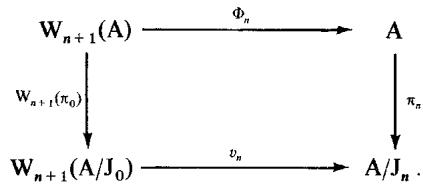
\includegraphics[keepaspectratio]{images/part002_309b7be5.jpg}}

\begin{enumerate}
\def\labelenumi{\alph{enumi})}
\setcounter{enumi}{2}
\tightlist
\item
  Set \(u_n = v_n \circ \mathbf{W}_{n+1}(\overline{\varphi}) \circ \mathbf{F}^{-n}\) Then, for every \(n \in \mathbf{N}\) , the following diagram, where the vertical arrows denote the canonical projections, is commutative
\end{enumerate}

\pandocbounded{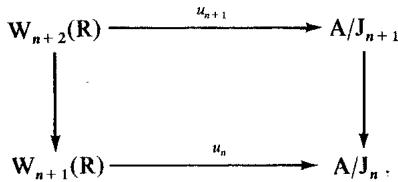
\includegraphics[keepaspectratio]{images/part002_feb0ecf4.jpg}}

\begin{enumerate}
\def\labelenumi{\alph{enumi})}
\setcounter{enumi}{3}
\tightlist
\item
  There exists a unique ring homomorphism u making the following diagram commutative.
\end{enumerate}

\pandocbounded{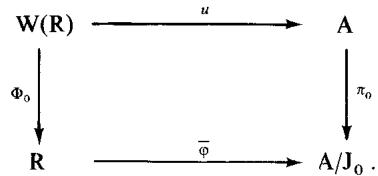
\includegraphics[keepaspectratio]{images/part002_890d1cac.jpg}}

  The homomorphism \(u\) is continuous when \(\mathbf{W}(\mathbf{R})\) is equipped with the \(p\)-adic topology, and for every \(\boldsymbol{a} = (a_n)_{n \in \mathbb{N}} \in \mathbf{W}(\mathbf{R})\), one has \(u(\boldsymbol{a}) = \sum_{n=0}^{\infty} p^n \varphi(a_n^{p^{-n}})\).

(The existence of \(u\) follows from what precedes. To prove the uniqueness of \(u\), its continuity, and its explicit expression, use the equality \(\varphi = u \circ \tau\), where \(\varphi\) is the map from R into A constructed in a), and \(\tau: \mathrm{R} \to \mathrm{W(R)}\) is the map defined in § 1, no. 5.)

\begin{enumerate}
\def\labelenumi{\alph{enumi})}
\setcounter{enumi}{4}
\tightlist
\item
  Give another proof of th. 2 of § 2, no. 4, different from the one in the text and from that of exerc. 4, c).
\end{enumerate}

\begin{enumerate}
\def\labelenumi{\arabic{enumi})}
\setcounter{enumi}{6}
\tightlist
\item
  \begin{enumerate}
  \def\labelenumii{\alph{enumii})}
  \tightlist
  \item
    Let R be a perfect ring of characteristic p, and let R' be a ring of characteristic p. Let f be a homomorphism from R into R'. Then the homomorphism W(f): W(R) → W(R') is the unique homomorphism making the following diagram commutative.
  \end{enumerate}
\end{enumerate}

\pandocbounded{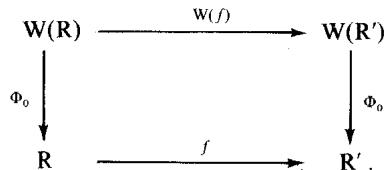
\includegraphics[keepaspectratio]{images/part002_f36acea2.jpg}}

(Use the previous exercise.)

In particular, taking \(f\) to be the p-th power map on R, prove that \(\mathrm{F}_{\mathrm{R}}\) is the unique endomorphism of \(\mathbf{W}(\mathbf{R})\) such that \(\Phi_{0} \circ \mathrm{F}_{\mathrm{R}} = f \circ \Phi_{0}\). It is characterized by the equalities

\[
\mathrm{F} _ {\mathbf {R}} (\tau (x)) = \tau (x ^ {p}) \quad \text { for all } \quad x \in \mathbf {R}  .
\]

\begin{enumerate}
\def\labelenumi{\alph{enumi})}
\setcounter{enumi}{1}
\tightlist
\item
  Let A be a ring separated and complete for the p-adic topology. Suppose that multiplication by \(p.1_{A}\) in A is injective and that A/pA is a perfect ring. Then there exists a unique endomorphism \(\sigma\) of A such that \(\sigma(x) \equiv x^{p} \mod pA\) for \(x \in A\), and the inverse of the isomorphism \(t_{\sigma}: A \to W(A/pA)\) described in exerc. 14, p.~44 is given by
\end{enumerate}

\[
(a _ {i}) _ {i \in \mathbf {N}} \mapsto \sum_ {i = 0} ^ {\infty} \varphi (a _ {i}) ^ {p ^ {- i}} p ^ {i},
\]

where \(\varphi : \mathrm{A} / p\mathrm{A} \to \mathrm{A}\) is the unique map which gives the identity of \(\mathrm{A} / p\mathrm{A}\) by passage to quotients and satisfies \(\varphi(x^p) = \varphi(x)^p\) for \(x \in \mathbb{R}\) (cf.~exerc. 6, a)).

\begin{enumerate}
\def\labelenumi{\arabic{enumi})}
\setcounter{enumi}{7}
\item
  Let C be a p-ring of infinite length, with residue field k. Every automorphism of k extends to an automorphism of C. Every automorphism of C inducing the identity on k by passage to quotients is the identity if and only if k is perfect.
\item
  Let \(k\) be a field of characteristic \(p\), \(\mathbf{C}_k\) a \(p\)-ring of infinite length and with residue field \(k\). Let A be a local ring separated and complete and \(u: \mathbf{C}_k \to \mathbf{A}\) a local homomorphism such that the homomorphism deduced from \(u\) by passage to quotients makes the residue field K of A a separable extension of \(k\). Let \(\mathbf{C}_{\mathbf{K}}\) be a \(p\)-ring of infinite length with residue field K. Prove that there exist local homomorphisms \(i: \mathbf{C}_k \to \mathbf{C}_{\mathbf{K}}\) and \(v: \mathbf{C}_{\mathbf{K}} \to \mathbf{A}\) such that \(u = v \circ i\) and that \(v\) induces the identity on K by passage to quotients.
\item
  Let \(k\) be a field of characteristic \(p\), \((\xi_{\lambda})_{\lambda \in \Lambda}\) a \(p\)-basis of \(k\), and for each integer \(n \geqslant 1\), let \(C_n\) be the subring of \(\mathbf{W}_n(k)\) generated by \(\mathbf{W}_n(k^{p^{n-1}})\) and the elements \(\tau(\xi_{\lambda}) = [\xi_{\lambda}, 0, ..., 0]\), for \(\lambda \in \Lambda\). For every integer \(n \geqslant 1\), the projection of \(\mathbf{W}_{n+1}(k)\) onto \(\mathbf{W}_n(k)\) maps \(C_{n+1}\) into \(C_n\). We denote by C the subring of \(\mathbf{W}(k)\) that is the inverse limit of the \(C_n\).
\end{enumerate}

\begin{enumerate}
\def\labelenumi{\alph{enumi})}
\item
  Let n be an integer \(\geqslant 0\). Put \(\mathbf{A} = \mathbf{W}_{n+1}(k)\) and for every integer \(i \geqslant 0\) let \(\rho_{i} = \rho_{n,i}^{A}\) be the map from k to A defined in exerc. 2, p.~69. Prove that one has, for \(a \in k\), \(\rho_{i}(a) = V^{i}\tau(a^{p^{n}})\). Deduce that the elements \(\rho_{i}(a)\) for \(a \in k\) generate the subring \(\mathbf{W}_{n+1}(k^{p^{n}})\) of A.
\item
  Let \(\tilde{\mathbf{C}}\) be a \(p\)-ring with residue field \(k\) and of infinite length, and let \((x_{\lambda})_{\lambda \in \Lambda}\) be a family of elements of \(\tilde{\mathbf{C}}\) lifting the \(p\)-basis \((\xi_{\lambda})_{\lambda \in \Lambda}\). Using exerc. 4, p.~70, prove that there exists, for each integer \(n \geqslant 1\), a unique ring homomorphism \(\varphi_n: \tilde{\mathbf{C}} \to \mathbf{W}_n(k)\) inducing the identity on \(k\) by passage to quotients, and sending \(x_{\lambda}\) onto \(\tau(\xi_{\lambda})\) for every \(\lambda \in \Lambda\). Deduce from exerc. 3, p.~69 that the image of \(\varphi_n\) is \(\mathbf{C}_n\).
\item
  The maps \((\varphi_n)_{n\geqslant 1}\) form an inverse system of maps from \(\tilde{\mathbf{C}}\) into the \(C_n\), and \(\varphi = \lim \varphi_n\) is an isomorphism from \(\tilde{\mathbf{C}}\) onto C. For each \(n\geqslant 1\), the canonical projection \(\mathbf{C}\to \mathbf{C}_n\) identifies \(C_n\) with \(\mathrm{C} / p^n\mathrm{C}\).
\end{enumerate}

\begin{enumerate}
\def\labelenumi{\arabic{enumi})}
\setcounter{enumi}{10}
\tightlist
\item
  Let \(k\) be a field of characteristic \(p\), \((\xi_{\lambda})_{\lambda \in \Lambda}\) a \(p\)-basis of \(k\), and \(C\) the Cohen subring of \(\mathrm{W}(k)\) containing \(\tau(\xi_{\lambda})\) for every \(\lambda \in \Lambda\). Let \((\varepsilon_j)_{j \in J}\) be a basis of \(k^*/(k^{*p})\) as an \(\mathbf{F}_p\)-vector space. Let \(n\) be an integer \(\geqslant 0\) and \((x_j)_{j \in J}\) be a family of elements of \(k^*\) such that the image of \(x_j\) in \(k^*/k^{*p}\) is \(\varepsilon_j\), for all \(j \in J\).
\end{enumerate}

\begin{enumerate}
\def\labelenumi{\alph{enumi})}
\item
  The group \(k^{*} / k^{*p^{n}}\) is a free \((\mathbf{Z} / p^{n}\mathbf{Z})\)-module with basis \((\overline{x}_j)_{j\in J}\), where \(\overline{x}_j\) is the class of \(x_j\) in \(k^{*} / k^{*p^{n}}\).
\item
  For every \(j \in J\), let us write the decomposition of \(x_{j}\) along the basis \((\xi^{m})_{m \in M_{n}}\) of k over \(k^{p^{n}}\) (with the notations of exerc. 3, p.~69):
\end{enumerate}

\[
x _ {j} = \sum_ {\boldsymbol {m} \in \mathbf {M} _ {n}} a _ {j, \boldsymbol {m}} ^ {p ^ {n}} \xi^ {\boldsymbol {m}}, \quad a _ {j, \boldsymbol {m}} \in k.
\]

Set

\[
\sigma_ {n} (x _ {j}) = \sum_ {m \in \mathbf {M} _ {n}} \tau (a _ {j, m} ^ {p ^ {n}} \xi^ {m}) \quad \text { for all } \quad j \in J
\]

and

\[
\sigma_ {n} (x) = \tau (x) \quad \text { for } \quad x \in k ^ {* p ^ {n}}.
\]

Then \(\sigma_{n}\) extends, in a unique way, to a multiplicative map from \(k^{*}\) into \(\mathrm{C} / p^{n + 1}\mathrm{C}\), still denoted \(\sigma_{n}\), which, by passage to quotients, determines the inclusion of \(k^{*}\) into \(k = \mathrm{C} / p\mathrm{C}\). c) Let \(\sigma_{n}^{\prime}\) be another multiplicative map from \(k^{*}\) into \(\mathrm{C} / p^{n + 1}\mathrm{C}\) defining the inclusion of \(k^{*}\) into \(k\) by passage to quotients. Then for every \(x\in k^{*}\), one has \(\sigma_{n}(x) = v(x)\sigma_{n}^{\prime}(x)\), where \(v\) is a homomorphism from \(k^{*}\) into the multiplicative group \((1 + p\mathrm{C}) / (1 + p^{n + 1}\mathrm{C})\) trivial on \(k^{*p^n}\). An arbitrary family \((\beta_j)_{j\in J}\) of elements of \(\mathrm{C} / p^n\mathrm{C}\) defines such a homomorphism by the formula

\[
v (x _ {j}) = 1 + p \beta_ {j} \quad \text { for all } \quad j \in J.
\]

\begin{enumerate}
\def\labelenumi{\alph{enumi})}
\setcounter{enumi}{3}
\item
  For every integer \(n \geqslant 0\) and every multiplicative map \(s_{n}: k^{*} \to C/p^{n+1}C\) defining the inclusion of \(k^{*}\) into k, passing to the quotient, there exists a multiplicative map \(s_{n+1}: k^{*} \to C/p^{n+2}C\) which determines \(s_{n}\) by passing to the quotient.
\item
  Prove that there exists a multiplicative section \(s:k\to C\). One can require that \(s(\xi_{\lambda})=\tau(\xi_{\lambda})\) for every \(\lambda\in\Lambda\).
\end{enumerate}

\(f)\) Let A be a local ring, separated and complete. Let \(k\) be its residue field, \((\xi_{\lambda})_{\lambda \in \Lambda}\) a \(p\)-basis of \(k\), and, for \(\lambda \in \Lambda\), let \(a_{\lambda}\) be a lifting of \(\xi_{\lambda}\) in A. Show that there exists a multiplicative section \(k^{*} \to A\) satisfying \(s(\xi_{\lambda}) = a_{\lambda}\).

\begin{enumerate}
\def\labelenumi{\arabic{enumi})}
\setcounter{enumi}{11}
\tightlist
\item
  Let A be a complete local ring whose residue field has characteristic p.
\end{enumerate}

\begin{enumerate}
\def\labelenumi{\alph{enumi})}
\item
  Let \(x \in \mathfrak{m}_{\mathrm{A}}\) . The map \(n \mapsto (1 + x)^n\) of \(\tilde{\mathbf{Z}}\) in \(1 + \mathfrak{m}_{\mathrm{A}}\) extends uniquely to a continuous map from \(\mathbf{Z}_p\) in \(1 + \mathfrak{m}_{\mathrm{A}}\) , denoted \(\alpha \mapsto (1 + x)^{\alpha}\) . This defines a structure of \(\mathbf{Z}_p\) -module on the multiplicative group \(1 + \mathfrak{m}_{\mathrm{A}}\) .
\item
  Let \(\delta\) be the formal series \(\exp\left(-\sum_{n=0}^{\infty}\mathrm{T}^{p^n}/p^n\right)\) of exercise 58, p.~68. The map \(x \mapsto \delta(x)\) from \(\mathfrak{m}_{\mathrm{A}}\) into \(1 + \mathfrak{m}_{\mathrm{A}}\) is bijective.
\item
  Let \(k\) be a perfect field of characteristic \(p\), and \(\varphi\) a local homomorphism from \(\mathbf{W}(k)\) into A. For \(\alpha \in \mathbf{W}(k)\), consider the series \(\varphi \mathrm{E}_{\mathrm{F}}(\alpha, \mathrm{T})\) obtained by applying \(\varphi\) to the coefficients of the series \(\mathrm{E}_{\mathrm{F}}(\alpha, \mathrm{T})\) from exercise 58, f), p.~68. For \(\alpha \in \mathbf{W}(k)\), \(x \in 1 + m_{\mathbf{A}}\), set \(x^{\alpha} = \varphi \mathrm{E}_{\mathrm{F}}(\alpha, \xi^{-1}(x))\). Show that this defines an action of the additive group \(\mathbf{W}(k)\) on the set \(1 + m_{\mathbf{A}}\), which extends the action of \(\mathbf{W}(\mathbf{F}_p)\) (identified with \(\mathbf{Z}_p\)) defined in a). Show that we also have, for \(a \in \mathbf{Z}_p\), \(\alpha \in \mathbf{W}(k)\), \(x \in 1 + m_{\mathbf{A}}\), the relation \((x^{\alpha})^{a} = x^{a\alpha}\).
\item
  Using exercise 15, p.~44, prove that one does not always have, for \(a \in \mathbf{Z}_{p}\), \(\alpha \in \mathbf{W}(k)\), and \(x \in 1 + m_{\mathbf{A}}\), the relation \((x^{a})^{\alpha} = x^{a\alpha}\). Nor do we always have, for \(\alpha \in \mathbf{W}(k)\) and \(x, y\) in \(1 + m_{\mathbf{A}}\), the relation \((xy)^{\alpha} = x^{\alpha}y^{\alpha}\).
\end{enumerate}

\begin{enumerate}
\def\labelenumi{\arabic{enumi})}
\setcounter{enumi}{12}
\tightlist
\item
  Let A be a complete discrete valuation ring of characteristic zero, whose residue field has characteristic \(p\). Let K be the field of fractions of A, \(\overline{\mathbf{K}}\) an algebraic closure of K, equipped with the unique valuation \(v\) extending that of K (VI, § 8, no. 7), \(\hat{\mathbf{K}}\) the completion of \(\overline{\mathbf{K}}\), \(\hat{\mathbf{A}}\) the valuation ring of \(\hat{\mathbf{K}}\). Put \(e = v(p)\).
\end{enumerate}

\begin{enumerate}
\def\labelenumi{\alph{enumi})}
\tightlist
\item
  The series \(\log(1 + x) = \sum_{i=1}^{\infty} (-1)^{i-1} x^i / i\) converges for \(v(x) > 0\) and defines homomorphisms of \(\mathbf{Z}_p\)-modules (cf. exerc. 12).
\end{enumerate}

\[
\begin{array}{l} \log : 1 + \mathfrak {m} _ {\hat {\mathbf {A}}} \to \hat {\mathbf {K}}, \\ \log : 1 + \mathfrak {m} _ {\mathbf {A}} \to \mathbf {K}. \end{array}
\]

\begin{enumerate}
\def\labelenumi{\alph{enumi})}
\setcounter{enumi}{1}
\tightlist
\item
  The series \(\exp(x) = \sum_{i=0}^{\infty} x^{i}/i!\) converges on the ideal \(a\) of \(\hat{K}\) consisting of elements of valuation \(>e/(p-1)\), and defines homomorphisms of \(\mathbf{Z}_{p}\)-modules
\end{enumerate}

\[
\begin{array}{l} \exp : a \to 1 + m _ {\hat {A}} \\ \exp : a \cap K \to 1 + m _ {A}. \end{array}
\]

\begin{enumerate}
\def\labelenumi{\alph{enumi})}
\setcounter{enumi}{2}
\tightlist
\item
  For \(x \in \mathfrak{a}\), one has \(\log(\exp(x)) = x\), \(\log(1 + x) \in \mathfrak{a}\), and \(\exp(\log(1 + x)) = 1 + x\). Thus exp defines isomorphisms of \(\mathbf{Z}_p\)-modules
\end{enumerate}

\[
\begin{array}{l}\mathfrak {a} \rightarrow 1 + \mathfrak {a}\\\mathfrak {a} \cap \mathbf {K} \rightarrow 1 + (\mathfrak {a} \cap \mathbf {K})\end{array}
\]

with inverses defined by log.

\begin{enumerate}
\def\labelenumi{\alph{enumi})}
\setcounter{enumi}{3}
\tightlist
\item
  The kernel of log on \(1 + m_{\hat{A}}\) consists of the roots of unity whose order is a power of p. The image \(\log(1 + m_{\hat{A}})\) is equal to \(m_{\hat{A}}\).
\end{enumerate}

\begin{enumerate}
\def\labelenumi{\arabic{enumi})}
\setcounter{enumi}{13}
\tightlist
\item
  Let A be a complete discrete valuation ring of characteristic zero, whose residue field \(k\) is perfect of characteristic \(p\). Let K be the field of fractions of A. Let \(n\) be an integer \(\geqslant 1\) and \(\zeta\) a primitive \(p^n\)-th root of unity in K. Let \(\overline{\mathbf{K}}\) be an algebraic closure of K, equipped with the unique valuation \(v\) extending that of K.
\end{enumerate}

\begin{enumerate}
\def\labelenumi{\alph{enumi})}
\item
  Let C be the Cohen subring of A, and T its field of fractions; this is a subfield of K. The canonical isomorphism from W(k) to C induces an isomorphism from \(W(k) \otimes_{\mathbb{Z}} \mathbb{Q}\) to T. For every finite extension l of k, the field \(W(l) \otimes_{\mathbb{Z}} \mathbb{Q}\) is a finite extension of \(W(k) \otimes_{\mathbb{Z}} \mathbb{Q}\), Galois if l is. If l is Galois, the unique extension \((T_l)\) of T in \(\overline{\mathbf{K}}\) isomorphic to \(W(l) \otimes_{\mathbb{Z}} \mathbb{Q}\) has residue field isomorphic to l. In particular, the field \(T_{\infty}\), the union of the fields \((T_l)\) as l ranges over the finite Galois extensions of k (in a fixed algebraic closure of k), has as its residue field an algebraic closure \(\overline{k}\) of k. The same holds for K. For each extension l of k in \(\overline{k}\), we denote by \((T_l)\) the unique extension of T in \(T_{\infty}\) whose residue field is the subfield l of \(\overline{k}\), and by \((K_l)\) the compositum of K and \((T_l)\). Then, if l is Galois over k, \((K_l)\) is Galois over K and its Galois group is canonically identified with the Galois group of l over k.
\item
  Let \(k_n\) be the largest abelian extension of \(k\) in \(\overline{k}\) whose Galois group is annihilated by \(p^n\). By virtue of Exercise 19, p.~45, we have a canonical isomorphism
\end{enumerate}

\[
\operatorname{Gal} (k _ {n} / k) \to \operatorname{Hom} (\mathrm{W} _ {n} (k) / \wp \mathrm{W} _ {n} (k), \mathbf {Z} / p ^ {n} \mathbf {Z}).
\]

By A, V, p.~85, th. 4, we have a canonical isomorphism

\[
\operatorname{Gal} \left(\mathrm{K} _ {k _ {n}} / \mathrm{K}\right)\rightarrow \operatorname{Hom} \left(\mathrm{H} _ {n} / \mathrm{K} ^ {* p ^ {n}}, \mu_ {p _ {n}} (\mathrm{K})\right)
\]

\(\text{where }\mathbf{H}_n = (\mathbf{K}_{\overline{k}}^*)^{p^n}\cap \mathbf{K}^*\)

Prove that there exists a unique mapping

\[
\mathrm{E} ^ {*}: \mathrm{W} _ {n} (k) / \wp \mathrm{W} _ {n} (k) \rightarrow \mathrm{H} _ {n} / \mathrm{K} ^ {* p ^ {n}}
\]

such that the following diagram is commutative:

\[
\begin{array}{c} \operatorname{Gal} (K _ {k _ {n}} / K) \xrightarrow {} \operatorname{Hom} (H _ {n} / K ^ {* p ^ {n}}, \mu_ {p ^ {n}} (K)) \\ \Bigg \downarrow \\ \operatorname{Gal} (k _ {n} / k) \xrightarrow {} \operatorname{Hom} (W _ {n} (k) / \wp W _ {n} (k), Z / p ^ {n} Z), \end{array}
\]

where the vertical arrow on the right denotes the map which, to the homomorphism \(\varphi\) of \(\mathbf{H}_n / \mathbf{K}^{*p^n}\) into \(\mu_{p^n}(\mathbf{K})\), associates the homomorphism \(\psi\) of \(\mathrm{W}_n(k) / \wp\mathrm{W}_n(k)\) into \(\mathbf{Z} / p^n\mathbf{Z}\) defined by \(\zeta^{\psi (\alpha)} = \varphi (\mathrm{E}^{*}(\alpha))\) for \(\alpha \in \mathrm{W}_n(k) / \wp\mathrm{W}_n(k)\). The map \(\mathrm{E}^*\) is an isomorphism.

\begin{enumerate}
\def\labelenumi{\arabic{enumi})}
\setcounter{enumi}{14}
\tightlist
\item
  Let us keep the hypotheses and notations of the preceding exercise.
\end{enumerate}

\begin{enumerate}
\def\labelenumi{\alph{enumi})}
\tightlist
\item
  Let \(\alpha \in \mathbf{W}(k)\) and \(\overline{\alpha} \in \mathbf{W}(\overline{k})\) be such that \(p(\overline{\alpha}) = \alpha\) (cf. p. 45, exerc. 19). Then the element \(\zeta^{p^{n\overline{\alpha}}}\) (p.~72, exerc. 12) of the completion \(\widehat{\mathbf{K}}\) of \(\overline{\mathbf{K}}\) depends only on \(\alpha\), belongs to \(\mathbf{K}\), and we have
\end{enumerate}

\[
v \left(\zeta^ {p ^ {n} \bar {\alpha}} - 1\right) \geqslant e p / (p - 1) \quad (\text { with } e = v (p)).
\]

(One may prove the equality

\[
\log \left(\zeta^ {p ^ {n} \overline {{{\alpha}}}}\right) = - p ^ {n} \sum_ {j = 1} ^ {\infty} \sum_ {\sigma = 0} ^ {j - 1} \left(\mathrm{F} ^ {\sigma} \alpha\right) \frac {\pi^ {p ^ {j}}}{p ^ {j}}
\]

\(\text{where }\pi = \delta^{-1}(\zeta)\) (loc. cit.) and where F denotes the Frobenius automorphism of \(\mathbf{W}(k)\).)

\begin{enumerate}
\def\labelenumi{\alph{enumi})}
\setcounter{enumi}{1}
\tightlist
\item
  For \(\alpha \in \mathbf{W}(k)\), denote by \(\mathrm{E}^{**}(\alpha)\) the class in \(\mathrm{K}^* / \mathrm{K}^{*p^n}\) of \(\zeta^{p^n\overline{\alpha}}\). Then \(\mathrm{E}^{**}(\alpha)\) equals 1 if \(\alpha \in p\mathbf{W}(k)\) or if \(\alpha \in p^n\mathbf{W}(k)\). The map from \(\mathrm{W}_n(k)/\wp\mathrm{W}_n(k)\) into \(\mathrm{K}^* / \mathrm{K}^{*p^n}\) which associates to the class of \(\alpha \in \mathbf{W}(k)\) the element \(\mathrm{E}^{**}(\alpha)\) takes its values in \(\mathrm{H}_n / (\mathrm{K}^*)^{p^n}\) and satisfies the conditions of exercise 14, b).
\end{enumerate}

\begin{enumerate}
\def\labelenumi{\arabic{enumi})}
\setcounter{enumi}{15}
\tightlist
\item
  Let A be a complete discrete valuation ring with residue field k.
\end{enumerate}

\begin{enumerate}
\def\labelenumi{\alph{enumi})}
\item
  Prove that there exists a multiplicative section \(\varphi:k^{*}\to\mathring{\mathrm{A}}\) (If A contains a field, use § 3. Otherwise, use exerc. 11, p.~72.)
\item
  Let \(t\) a uniformizer of A, \(\mathcal{C}\) the group generated by \(t\) , and \(\varphi:k^{*}\to A\) a multiplicative section. The multiplicative group of the field of fractions of A decomposes as a direct product. \(\mathcal{C}\times\varphi(k^{*})\times(1+\mathfrak{m}_{\mathbf{A}})\) .
\item
  Suppose A has equal characteristics and let K be a coefficient field. Then A is identified with the ring K{[}{[}T{]}{]} formal series with coefficients in K, and the group 1 + m\_A is identified with the group \(\Lambda(K) = 1 + TK[[T]]\) (cf. p. 56, exerc. 42). If K has characteristic zero, the map \(\varphi \mapsto \frac{1}{T} \log \varphi\) of the group \(\Lambda(K)\) in the additive group \(K[[T]]\) is an isomorphism. If A has characteristic \(p, 1 + m_A\) is identified with the group \(W(A)^L\) where L is the set of positive integers coprime to \(p\) (using Exercises 40, \(h\) ) p.~54 and 43, \(b\) ), p.~57).
\end{enumerate}

\begin{enumerate}
\def\labelenumi{\arabic{enumi})}
\setcounter{enumi}{16}
\tightlist
\item
  Let A be a complete discrete valuation ring whose residue field k is perfect of characteristic p and whose fraction field is of characteristic 0. Let f be the unique homomorphism from W(k) to A that induces the identity on the residue field k. Finally, let π be a uniformizer of A.
\end{enumerate}

\begin{enumerate}
\def\labelenumi{\alph{enumi})}
\item
  There exists an Eisenstein polynomial P with coefficients in \(f(\mathbf{W}(k))\) such that \(\mathbf{P}(\pi)=0\) (use VIII, § 5, no. 4).
\item
  Let \(e\) be the valuation of \(p\). For every integer \(n \geqslant 0\), denote by \(U_n\) the multiplicative group \(1 + m_A^n\), and set \(\lambda(n) = \inf(np, n + e)\), \(e_1 = e/(p - 1)\). Let \(u\) be the class in \(k^*\) of \(p\pi^{-e}\). Let \(\varphi\) be the endomorphism of \(U_1\) which sends \(x\) to \(x^p\). We then have, for every integer \(n \geqslant 1\), \(\varphi(U_n) \subset U_{\lambda(n)}\), \(\varphi(U_{n+1}) \subset U_{\lambda(n)+1}\), and the induced homomorphism \(\varphi_n: U_n/U_{n+1} \to U_{\lambda(n)}/U_{\lambda(n)+1}\) is an isomorphism if \(n \neq e_1\). If \(n = e_1\), \(\varphi_n\) is injective if and only if the equation \(x^{p-1} + u = 0\) has no solution in \(k\), and surjective if and only if the equation \(x^p + ux = y\) has a solution in \(k\) for every \(y \in k\).
\item
  The following two conditions are equivalent:
\end{enumerate}

\begin{enumerate}
\def\labelenumi{(\roman{enumi})}
\item
  A contains the p-th roots of unity;
\item
  \(e_1\) is an integer and the equation \(x^{p - 1} + u = 0\) has a solution in \(k\) .
\end{enumerate}

\begin{enumerate}
\def\labelenumi{\alph{enumi})}
\setcounter{enumi}{3}
\item
  The topology induced on \(\mathbf{U}_1\) by that of A coincides with the p-adic topology of \(\mathbf{U}_1\).
\item
  Let S be the set of integers \(n \geqslant 1\) such that A contains the \(p^n\)-th roots of unity. Then \(s = \text{Card}(S)\) is finite.
\item
  Let I be the set of integers \(i\) coprime to \(p\) and satisfying \(1 \leqslant i < e + e_1\). Then we have Card(I) = \(e\), and the image of \(\mathbf{N} - \{0\}\) by \(\lambda\) is \(\mathbf{N} - (\mathbf{I} \cup \{0\})\).
\item
  If \(e_1\) is an integer and \(\varphi_{e_1}\) is not surjective, set \(\mathbf{I}' = \mathbf{I} \cup \{e + e_1\}\); otherwise, set \(\mathbf{I}' = \mathbf{I}\). For each integer \(i \in \mathbf{I}'\), let \(\pi_i\) be an element of A with valuation \(i\). Then the map from \(\mathbf{W}(k)^{\mathbf{I}'}\) into \(\mathbf{U}_1\) which sends \((a_i)_{i \in \mathbf{I}'}\) to \(\prod_{i \in \mathbf{I}'} (1 + \pi_i)^{a_i}\) is surjective; it is a homomorphism of
\end{enumerate}

\(\mathbf{Z}_{p}\)-modules.

\(h)\) Let \(n\) be an integer \(>e_{1}\) and \(\mathbf{I}(n)\) the interval \([n, \lambda(n) - 1]\) of \(\mathbf{N}\). For every integer \(i \in \mathbf{I}(n)\), let \(\pi_{i}\) be an element of \(\mathbf{A}\) of valuation \(i\). Then the map from \(\mathbf{W}(k)^{\mathbf{I}(n)}\) into \(\mathbf{U}_{n}\) which sends \((a_{i})_{i \in \mathbf{I}(n)}\) to \(\prod_{i \in \mathbf{I}(n)} (1 + \pi_{i})^{a_{i}}\) is an isomorphism of \(\mathbf{Z}_{p}\)-modules.

\begin{enumerate}
\def\labelenumi{\roman{enumi})}
\tightlist
\item
  Suppose that \(k\) is finite and denote by \(d\) the degree over \(\mathbf{Q}_{p}\) of the field of fractions of A. Then the \(\mathbf{Z}_{p}\)-module \(1 + m_{\mathbf{A}}\) is isomorphic to \((\mathbf{Z}/p^{s}\mathbf{Z}) \times \mathbf{Z}_{p}^{d}\) (One may use the preceding questions, or else use Exercise 13, p.~73.)
\end{enumerate}

